\chapter{Proyecciones futuras (SSP5-8.5, 2040–2074)}\label{cap:5}

La segunda pregunta es si, bajo SSP5-8.5, cambia la probabilidad de rachas prolongadas ---no solo el acumulado anual. La comparación es ALADIN histórico versus ALADIN futuro, con el mismo R₀. A escala de Chile, el modelo proyecta menos precipitación anual en el centro-sur (del orden de −10 a −20 \% en gran parte del dominio) y, a la vez, un aumento de la duración media de dry spells de varios días en el norte y el centro (Figura~\ref{fig:mapas_futuro}).

\begin{figure}[htbp]
\centering
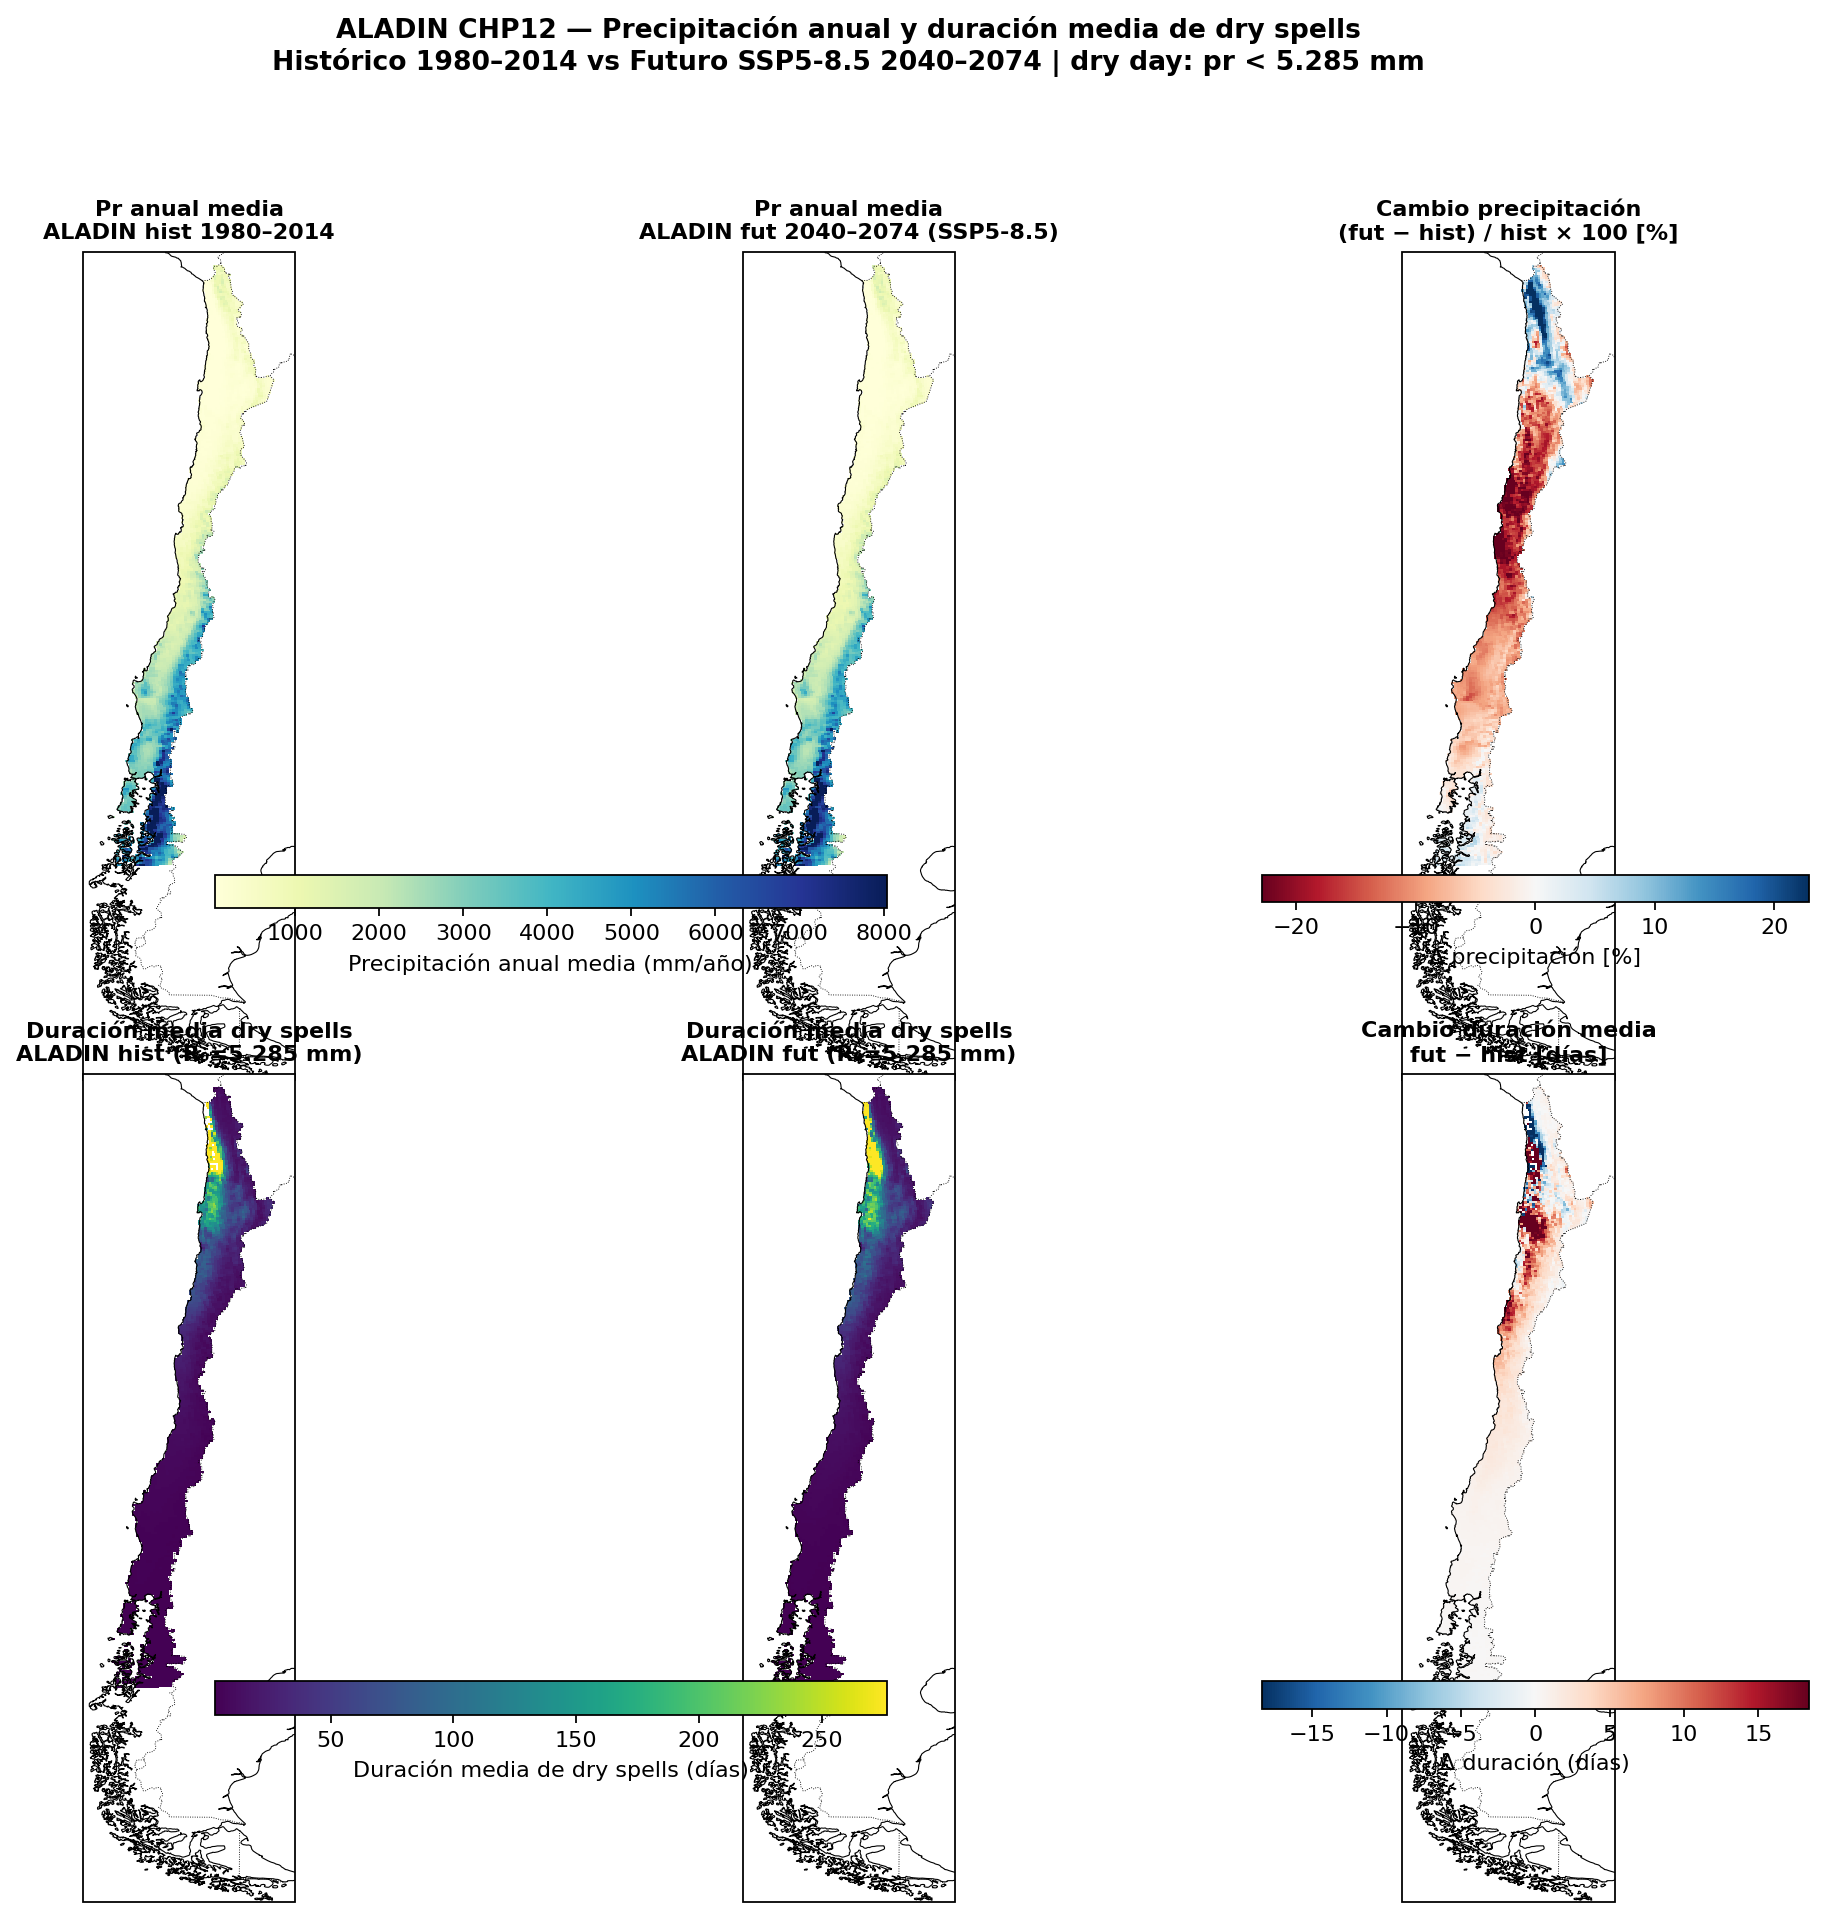
\includegraphics[width=1\linewidth,height=0.72\textheight,keepaspectratio,alt={ALADIN CHP12, criterio i. Fila superior: precipitación anual media en 1980--2014, 2040--2074 (SSP5-8.5) y cambio relativo (\%). Fila inferior: duración media de dry spells en ambos períodos y diferencia absoluta (días). El centro-sur pierde lluvia anual y alarga las rachas secas; no es un simple reescalado de la media de precipitación.}]{mapas_aladin_pr_anual_y_dryspells_hist_fut.png}
\caption[Precipitación anual y duración media de dry spells en ALADIN, histórico y futuro]{ALADIN CHP12, criterio i. Fila superior: precipitación anual media en 1980--2014, 2040--2074 (SSP5-8.5) y cambio relativo (\%). Fila inferior: duración media de dry spells en ambos períodos y diferencia absoluta (días). El centro-sur pierde lluvia anual y alarga las rachas secas; no es un simple reescalado de la media de precipitación.}\label{fig:mapas_futuro}
\end{figure}

\section{Risk ratios: más dry spells largos}\label{sec:rr_res}

El risk ratio RR(D) = N\_fut(t ≥ D) / N\_hist(t ≥ D) se estima en pools de regiones administrativas, con spells de inicio en marzo--noviembre y bootstrap por años (Figura~\ref{fig:rr}; Tabla~\ref{tab:rr}). A D = 20 días, Coquimbo pasa de 25 367 a 28 458 spells largos (RR = 1,12; IC95 {[}1,01, 1,25{]}); La Araucanía, de 2 397 a 4 118 (RR = 1,72; {[}1,10, 2,88{]}). En esas dos regiones el IC95 queda por completo sobre 1: el aumento es significativo. O'Higgins tiene RR = 1,15 (7 015 → 8 096), pero el IC95 {[}0,95, 1,40{]} cruza 1; aunque el RR es mayor que 1 en toda la cola, el intervalo solo queda marginalmente sobre 1 a D = 60 días (RR = 1,49; {[}1,01, 2,22{]}), por lo que no se interpreta como un aumento robusto. Los Lagos tiene RR = 2,15 (601 → 1 291), pero el IC95 {[}0,90, 8,50{]} cruza 1: el cociente es inestable porque los spells ≥ 20 días son raros en el histórico.

La señal no es un desplazamiento uniforme de toda la distribución. En Coquimbo, a D = 5 días el RR de conteos es 0,94 (IC95 por debajo de 1): hay menos spells cortos, coherente con la caída de n\_spells. El aumento es significativo a D = 20 días y de forma sostenida entre 30 y 60 días (p.~ej. RR = 1,26 a D = 30 días, IC95 {[}1,10, 1,43{]}). En La Araucanía el RR crece con D y alcanza 3,47 a 30 días, con IC95 amplio ({[}1,29, 11,8{]}): hay más ocurrencia de spells largos, pero la rareza histórica infla el cociente. Eso es lo que un CDD anual no muestra: el cambio está en la frecuencia de excedencias a lo largo de la cola, no en un único máximo por año (Sillmann et al., 2013b; Wainwright et al., 2021).

\begin{longtable}[]{@{}cccccc@{}}
\caption[Risk ratio a D = 20 días por región (SSP5-8.5)]{Risk ratio a D = 20 días. RR = N\_fut(t ≥ 20) / N\_hist(t ≥ 20). ALADIN, R₀ = 5,285 mm, inicio marzo--noviembre. IC95 por bootstrap de años (1 000 réplicas).}\label{tab:rr}\tabularnewline
\toprule\noalign{}
Región & N\_hist (t≥20) & N\_fut (t≥20) & RR & IC95 & ¿Aumento sig.? \\
\midrule\noalign{}
\endfirsthead
\toprule\noalign{}
Región & N\_hist (t≥20) & N\_fut (t≥20) & RR & IC95 & ¿Aumento sig.? \\
\midrule\noalign{}
\endhead
\bottomrule\noalign{}
\endlastfoot
Coquimbo & 25367 & 28458 & 1,12 & {[}1,01, 1,25{]} & Sí \\
O'Higgins & 7015 & 8096 & 1,15 & {[}0,95, 1,40{]} & No (IC cruza 1) \\
La Araucanía & 2397 & 4118 & 1,72 & {[}1,10, 2,88{]} & Sí \\
Los Lagos & 601 & 1291 & 2,15 & {[}0,90, 8,50{]} & No (IC cruza 1) \\
\end{longtable}

\begin{figure}[htbp]
\centering
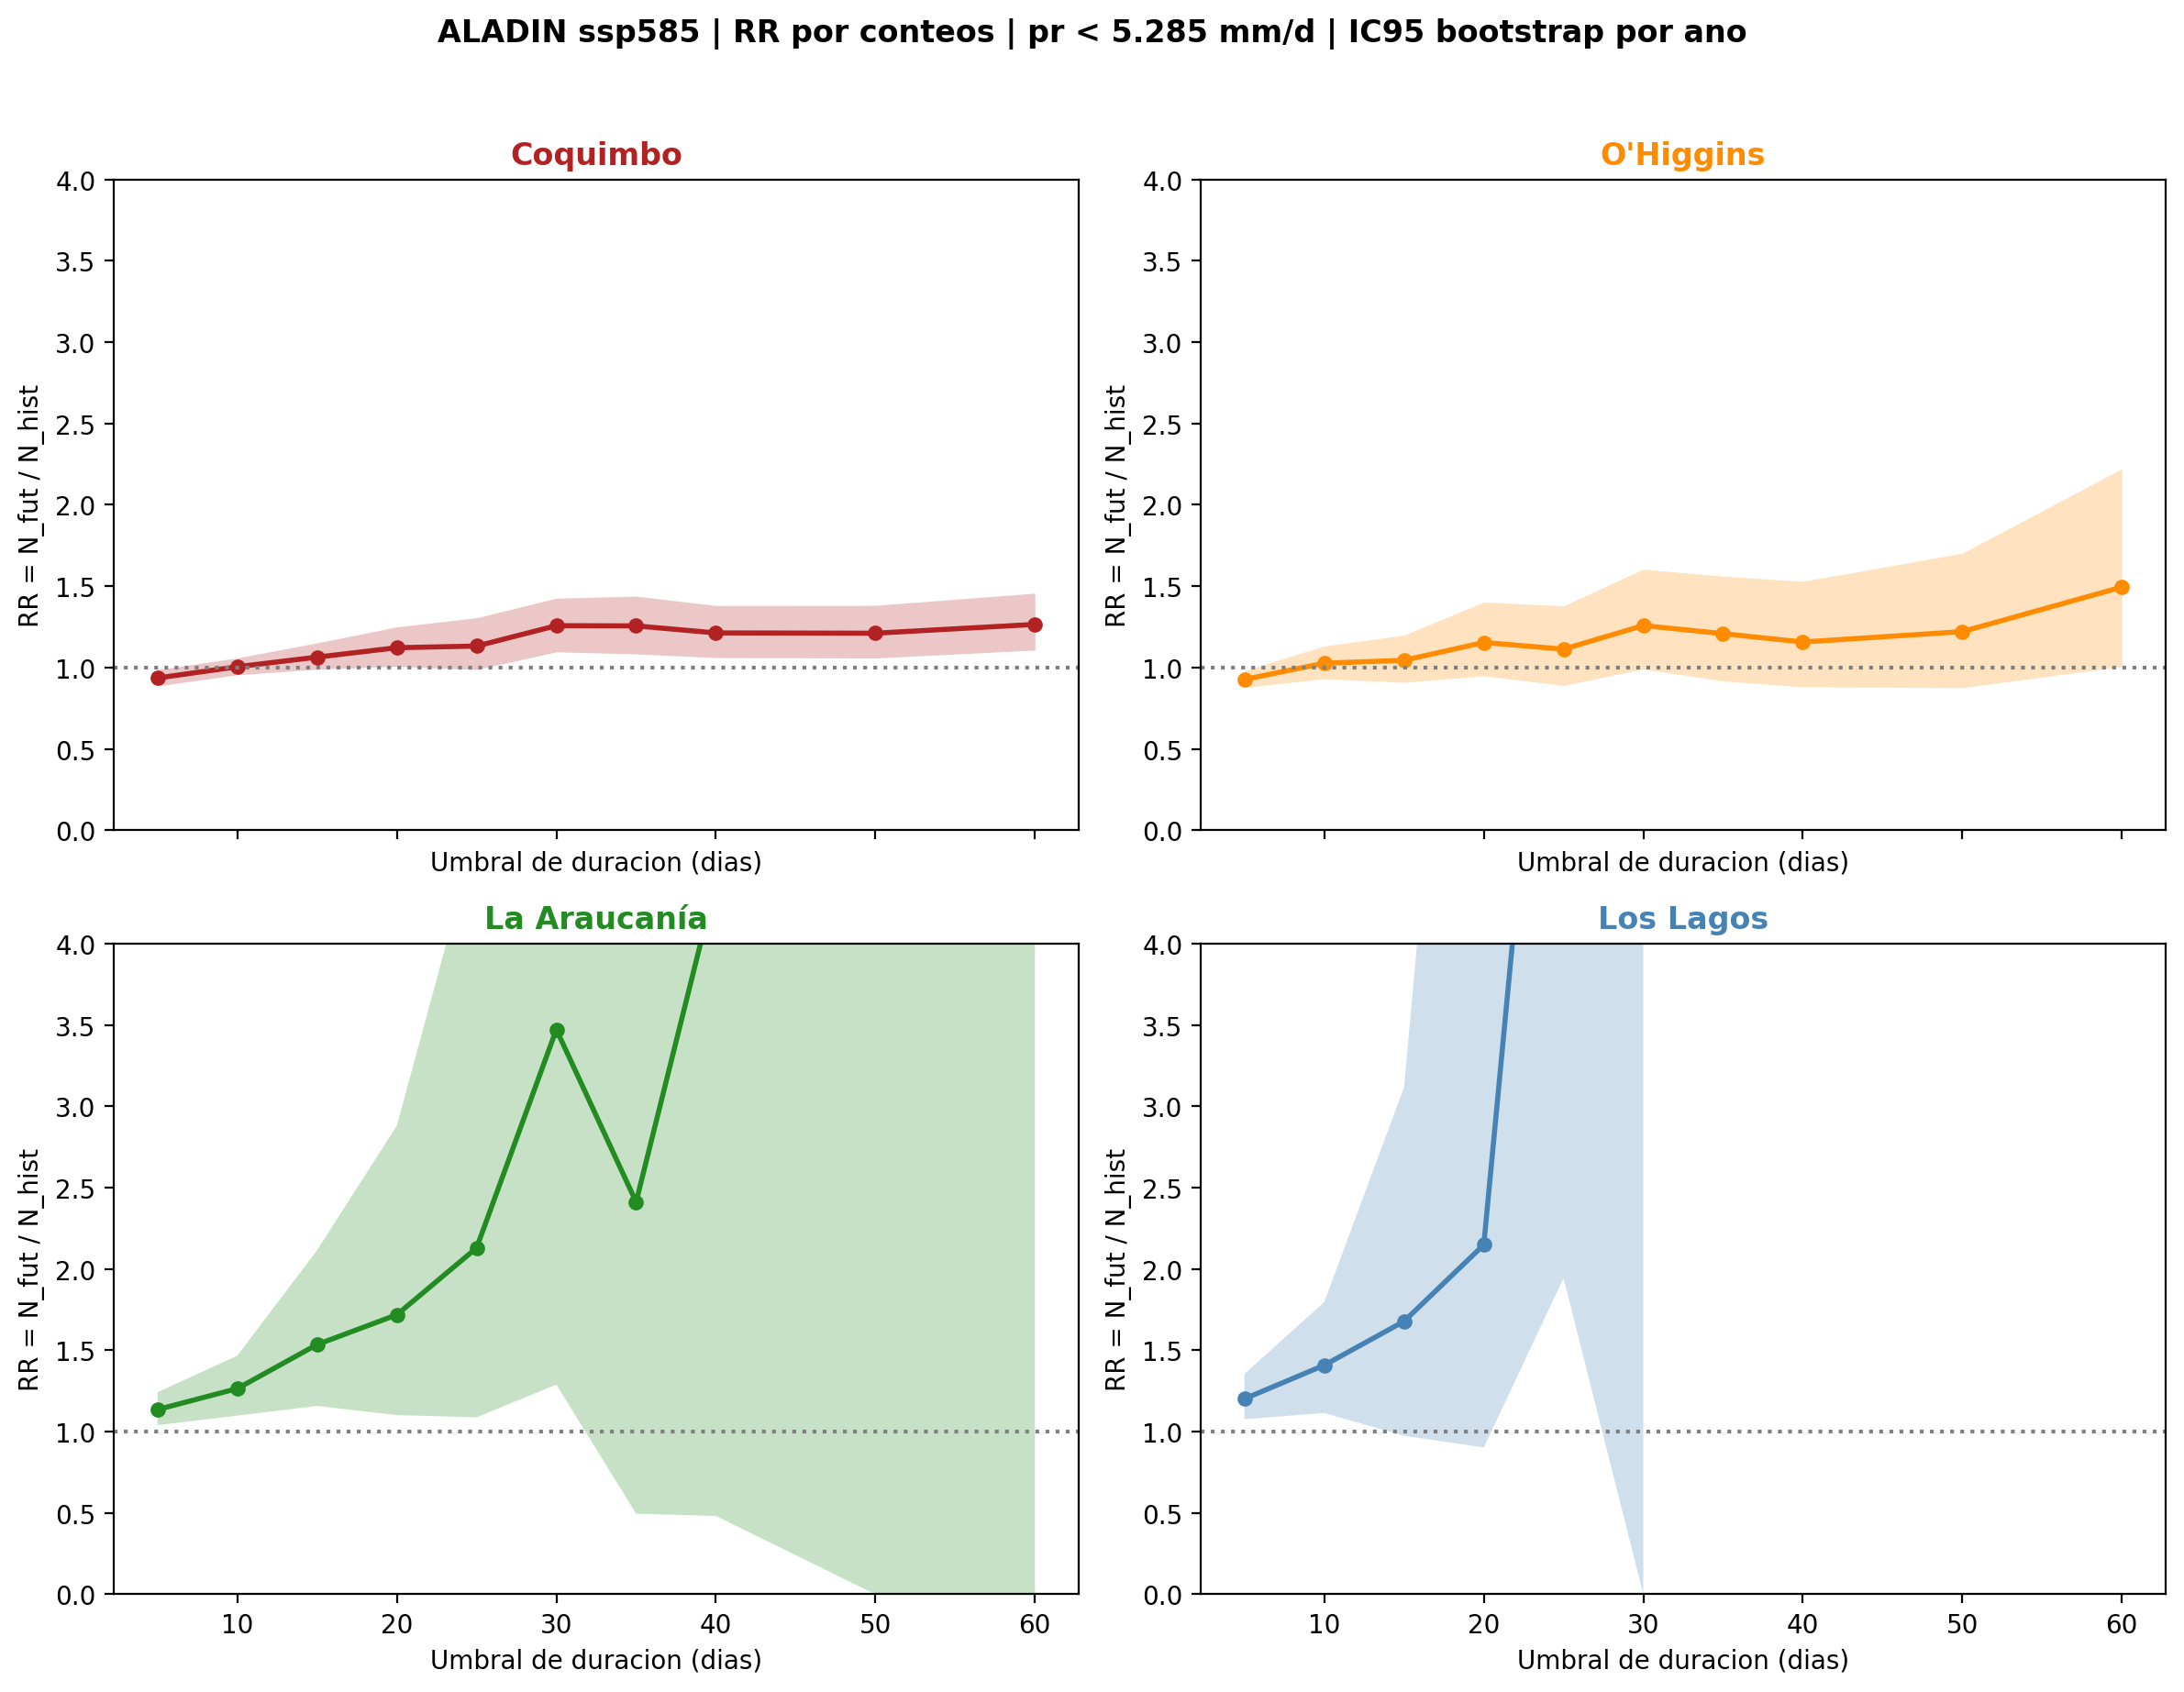
\includegraphics[width=1\linewidth,height=0.72\textheight,keepaspectratio,alt={Risk ratio RR(D) = N\_fut(t ≥ D) / N\_hist(t ≥ D) de dry spells con duración al menos D días. ALADIN, SSP5-8.5 (2040--2074) respecto de 1980--2014, R₀ = 5,285 mm, inicio marzo--noviembre. La banda es el IC95 por bootstrap de años. La línea punteada marca RR = 1. Coquimbo y La Araucanía superan 1 con IC que no cruza 1 a D = 20 días; O'Higgins y Los Lagos no. En el sur la banda se abre cuando D crece y los eventos históricos escasean.}]{fig08_rr_curves_aladin.png}
\caption[Risk ratio RR(D) = N\_fut(t ≥ D) / N\_hist(t ≥ D) de dry spells con duración al menos D días]{Risk ratio RR(D) = N\_fut(t ≥ D) / N\_hist(t ≥ D) de dry spells con duración al menos D días. ALADIN, SSP5-8.5 (2040--2074) respecto de 1980--2014, R₀ = 5,285 mm, inicio marzo--noviembre. La banda es el IC95 por bootstrap de años. La línea punteada marca RR = 1. Coquimbo y La Araucanía superan 1 con IC que no cruza 1 a D = 20 días; O'Higgins y Los Lagos no. En el sur la banda se abre cuando D crece y los eventos históricos escasean.}\label{fig:rr}
\end{figure}

\section{PDFs por cuenca: extensión de la cola futura}\label{sec:pdfs_fut}

Las PDFs de la Figura~\ref{fig:pdfs}, leídas ahora en la curva futura, muestran el cambio de forma y de n\_spells. En las cuatro cuencas el futuro de ALADIN tiene menos spells que el histórico: hay menos interrupciones y, por tanto, rachas más largas. La señal es clara en Maipo--Maule--Biobío, donde suben la media y el p99 y la cola se extiende hacia duraciones de decenas a cientos de días; en Loa el cambio relativo es menor porque las rachas ya son prolongadas (Tabla~\ref{tab:estadisticos}; Figura~\ref{fig:pdfs}). En escala log--log las curvas no son una traslación paralela: el exceso futuro se concentra a la derecha.

El máximo muestral es un estadístico ruidoso y no debe usarse solo. En Biobío, por ejemplo, el máximo del pool baja aunque media, p90, p99 y la probabilidad de spells ≥ 20 días suben. Eso ilustra por qué el objeto del trabajo es la distribución y las excedencias, no el récord de un píxel.

En conjunto, los risk ratios y las distribuciones de duración muestran un alargamiento de los dry spells hacia mediados de siglo, concentrado especialmente en la cola en Chile central y centro-sur. El cambio relativo es pequeño en Loa, donde las rachas ya son prolongadas en el histórico, mientras que en Los Lagos la estimación de la cola permanece incierta por la rareza de eventos largos.

\pendiente{decidir si las sensibilidades S4 (umbral) y S6 (SSP3-7.0) del Anexo A se
integran aquí como sección de robustez.}
